\chapter{Pointers} % (fold)
\label{chap:Pointers}
\section{Pointer Variables} % (fold)
\label{sec:Pointer Variables}
\begin{Definition}[colbacktitle=red!75!black]{Address}{}
The values of variables are stored in the computer's memory, each at a particular location. Each location is identified and referenced with an \textbf{address}.
\end{Definition}

\begin{Definition}[colbacktitle=red!75!black]{Pointer, Pointer variable}{}
\textbf{Pointer variable} is a \underline{variable} whose \underline{value is the address of some other memory location}.
\end{Definition}


% section Pointer Variables (end)
\section{Memory and Addresses} % (fold)
\label{sec:Memory and Addresses}

\begin{figure}[H] %h:当前位置, t:顶部, b:底部, p:浮动页
  \centering
  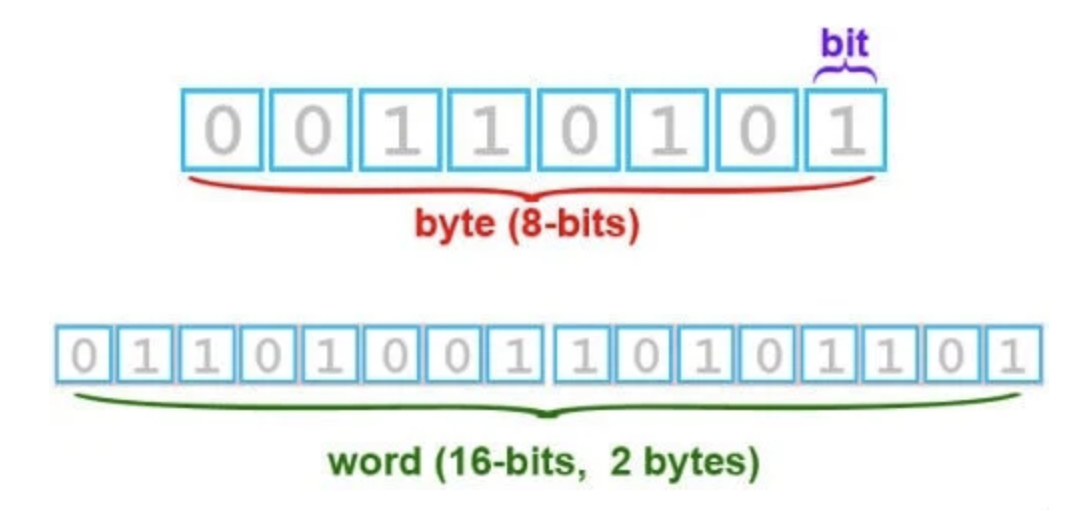
\includegraphics[width=0.5\textwidth]{./assets/Bits and Bytes.png}
  \caption{Bits and Bytes}
  \label{fig:Bits and Bytes}
\end{figure}

\begin{Definition}[colbacktitle=red!75!black]{Bits, Bytes, Words}{}
Computer memories are composed of 
\begin{itemize}

    \item \textbf{bits}, each capable of holding either the value 0 or the value 1.

    \item \textbf{bytes}, grouping together \textbf{bits} and treated as a unit in order to store a wider range of values. Usually, each \textbf{bytes} contains eight \textbf{bits}, storing unsigned integers from 0 to 255 or signed integers from -128 to 127.

    \item \textbf{words}, taking two or more \textbf{bytes} and treat them as if they were a \underline{single}, larger unit of memory, in order to store even larger values.

\end{itemize}

Note : Even though a word contains 4 bytes, it has only one address.
\end{Definition}

\begin{Prop}{Location in memory}{}

  \begin{enumerate}

      \item Each location in memory is identified by a unique address. 
      \item Each location in memory contains a value.

  \end{enumerate}
\end{Prop}

\begin{Prop}{Address versus contents}{}
  \begin{itemize}

      \item As it is difficult to remember the real addresses, the high-level languages provide the ability to refer to memory locations by name (\textbf{variables}) rather than by address. This is done by the \textit{compiler}.

      \item The \textit{hardware} still accesses memory locations using addresses.

  \end{itemize}
\end{Prop}

% section Memory and Addresses (end)



% section Contents of a Pointer Value (end)
\section{Declaration and Initialization} % (fold)
\label{sec:Declaration and Initialization}



\subsection{Passing the address to the pointer, Indirection the pointer} % (fold)
\label{sub:Declaring Pointers}

\begin{Prop}{Declaration}{}
See the code :
\begin{lstlisting}
int *a; // Declaration : a pointer to an integer.
float *a;
\end{lstlisting}
\end{Prop}
\begin{Prop}{Initialization of a pointer variable}{}
Pointers are initialized with the \textit{addresses of other variables}.  \verb|&| operator produces the memory address of its operand.

\end{Prop}

\begin{Definition}[colbacktitle=red!75!black]{Indirection or dereferencing the pointer}{}
The process of following a pointer to the location  to which it points \underline{to obtain the value} is called \textbf{Indirection} or \textbf{dereferencing} the pointer. 

The operator is the unary \verb|*|. 
\end{Definition}



When declaring two or more pointers:
\begin{lstlisting}
int *a, *b, *c; // Correct 
int *a,  b,  c; // Wrong, two integers with one pointer
\end{lstlisting}

Declaration with initialization :
\begin{lstlisting}
int a; 
int *d = &a; 

char *message = "Hello world!";
// The value is assigned to message (the pointer variable) rather than *message
// It equals to : 
char *message; 
message = "Hello world!";
\end{lstlisting}
% subsection Declaration (end)
% section Initialization (end)

\subsection{Values and their Types} % (fold)
\label{sec:Values and their Types}

\begin{Prop}{Type of a value and the value itself}{}
The type of a value is not something inherent in the value itself but depends on how it is used. The type of a value cannot be determined simply by examining its bits. 
\end{Prop}



Thus, declaring a variable to be a \verb|float| causes the compiler to generate \textit{floating-point instructions} when accessing it. 

\begin{lstlisting}
// Two ways of pointing according to the type of the value.
int    a = 112, b = -1;
int   *c = &a;

float   d = 3.14;
float  *e = &d;
\end{lstlisting}

% section Values and their Types (end)

\subsection{Uninitialized and Illegal Pointer} % (fold)
\label{sub:Uninitialized and Illegal Pointer}
A very common error :

\begin{lstlisting}
int  *a; 
... 
*a = 12; 
/* We're goint to assign the value 12 in the location where a points to. 
 * But where does a points to exactly ? */
\end{lstlisting}

Don't access a location that is outside of the memory allocated to your program. (\textbf{Bus error})
% subsection Uninitialized and Illegal Pointer (end)

\subsection{Null Pointer} % (fold)
\label{sub:Null Pointer}

\begin{Definition}[colbacktitle=red!75!black]{NULL pointer}{}
A \textbf{NULL pointer} is a pointer value that does not point to anything at all.
\end{Definition}

To make a pointer variable \verb|NULL| assign the value zero. 

To test a pointer variable is \verb|NULL| you compare it to zero.



% subsection Null Pointer (end)

\section{Contents of a Pointer Value, Indirection Operator} % (fold)
\label{sec:Contents of a Pointer Value}





\begin{lstlisting}
float *e = &d;  
/* 1. Produce the memory address of d 
 * 2. Pass the value to which we dereference a pointer */ 
\end{lstlisting}

\begin{Prop}{Contents of a pointer variable}{}
The contents of pointers are \underline{addresses}  rather than integers or floating-point numbers. 

It is important to distinguish between the address of the variable and its contents.
\end{Prop}

% chapter Pointers (end)
